\newpage
\subsection{Caso d'uso UC20: Recupera password}
\label{UC20}
\begin{figure}
	\centering
	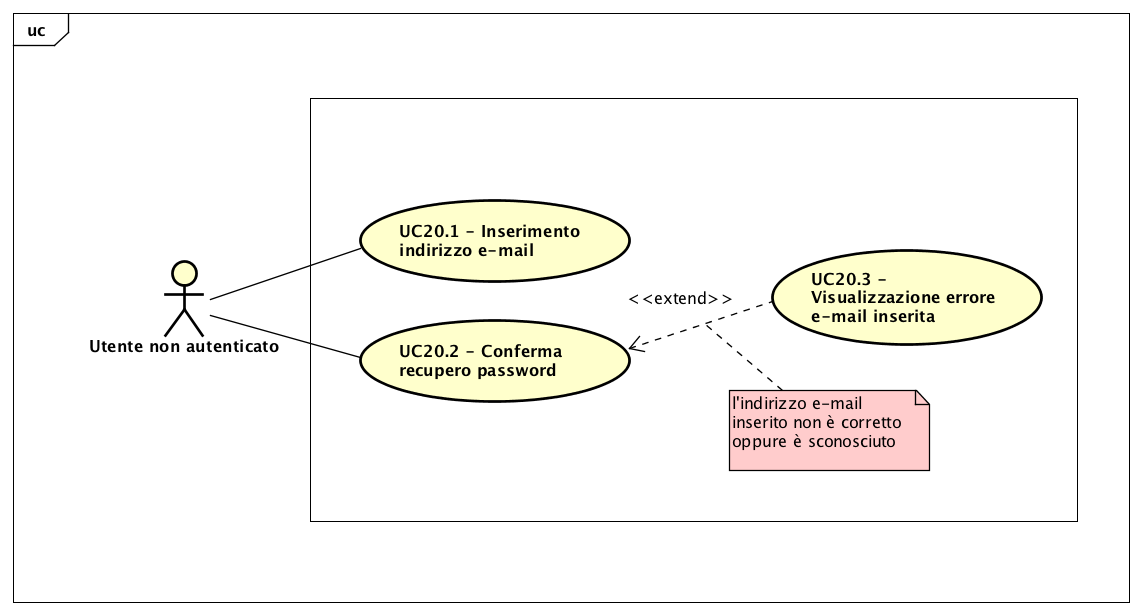
\includegraphics[scale=0.48]{UML/UC20.png}
	\caption{UC20: Recupera password}
\end{figure}
\FloatBarrier
\begin{itemize}
	\item \textbf{Attori}: utente non autenticato;
	\item \textbf{Descrizione}: l'attore può recuperare la propria password se dimenticata;
	\item \textbf{Precondizione}: il sistema è avviato e pronto per l'utilizzo e mostra la pagina di login;
	\item \textbf{Postcondizione}: il sistema ha inviato una mail all'indirizzo dell' iscrizione dell'attore;
	\item \textbf{Scenario Principale}:
	\begin{enumerate}
		\item L'attore può inserire la e-mail utilizzata al momento della registrazione (UC20.1);
		\item L'attore può confermare il recupero della password (UC20.2);
	\end{enumerate}
	\item \textbf{Estensioni}: indirizzo e-mail non valido oppure sconosciuto (UC20.3).
\end{itemize}

\subsubsection{Caso d'uso UC20.1: Inserimento indirizzo e-mail}
\begin{itemize}
	\item \textbf{Attori}: utente non autenticato;
	\item \textbf{Descrizione}: l'attore può inserire la e-mail associata al proprio account;
	\item \textbf{Precondizione}: il sistema presenta all'attore lo spazio destinato a questa operazione;
	\item \textbf{Postcondizione}: l'attore ha inserito la propria e-mail con cui è registrato;
	\item \textbf{Scenario principale}: l'attore inserisce la mail associata al proprio account. 
\end{itemize}

\subsubsection{Caso d'uso UC20.2: Conferma recupero password}
\begin{itemize}
	\item \textbf{Attori}: utente non autenticato;
	\item \textbf{Descrizione}: l'attore può confermare il recupero della password;
	\item \textbf{Precondizione}: l'attore ha inserito la e-mail;
	\item \textbf{Postcondizione}: il sistema invia una e-mail con la password all'indirizzo e-mail inserito dall'attore;
	\item \textbf{Scenario principale}: l'attore conferma il recupero password.
\end{itemize}

\subsubsection{Caso d'uso UC20.3: Visualizzazione errore e-mail inserita}
\begin{itemize}
	\item \textbf{Attori}: utente non autenticato;
	\item \textbf{Descrizione}: l'attore può visualizzare un messaggio d'errore nel caso si fossero verificati uno o più scenari alternativi durante la fase di recupero della password;
	\item \textbf{Precondizione}: il sistema ha ricevuto dei dati errati per il recupero password;
	\item \textbf{Postcondizione}: il sistema avvisa l'attore dell'errore verificatosi tramite un opportuno messaggio;
	\item \textbf{Scenario principale}: l'attore visualizza un messaggio d'errore.
\end{itemize}